\uuid{5Wyx}
\exo7id{7126}
\titre{exo7 7126}
\auteur{megy}
\organisation{exo7}
\datecreate{2017-02-08}
\isIndication{true}
\isCorrection{true}
\chapitre{Géométrie affine euclidienne}
\sousChapitre{Géométrie affine euclidienne du plan}
\module{Géométrie}
\niveau{L2}
\difficulte{}

\contenu{
\texte{
% Mettre l'autre sens
% points cocycliques
Soit $ABC$ un triangle direct, et $P$, $Q$ $R$ trois points situés sur $[BC]$, $[CA]$ et $[AB]$ respectivement, et distincts des sommets. Montrer que les cercles circonscrits à $ARQ$, $BPR$ et $CQP$ sont concourants.

\begin{center}
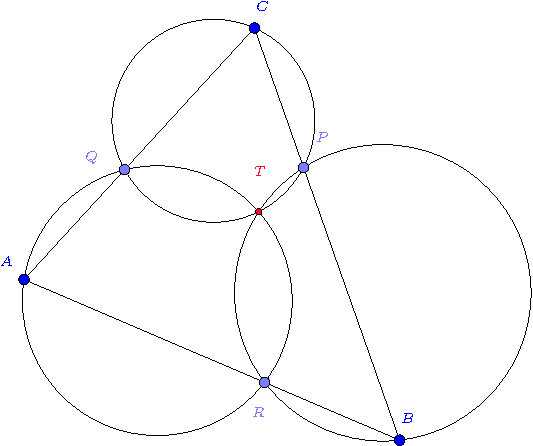
\includegraphics{../images/5Wyx-1}
\end{center}
}
\indication{Soient $\mathcal C$ et $\mathcal C'$ les cercles circonscrits à $ARQ$ et $BPR$. 
Ils se coupent en $R$ et en un deuxième point $T$, ou alors ils sont tangents en $R$. Montrer que $T$ (ou $R$ dans le second cas) est sur le cercle circonscrit à $CQP$.}
\reponse{
Soient $\mathcal C$ et $\mathcal C'$ les cercles circonscrits à $ARQ$ et $BPR$. 
Traitons le premier cas, celui où ils se coupent en $R$ et en un deuxième point $T$.

\begin{center}
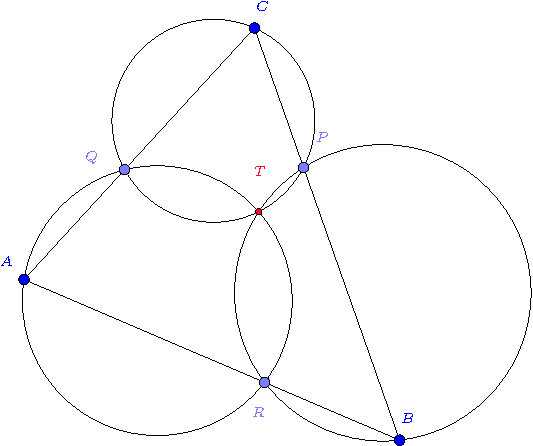
\includegraphics{../images/5Wyx-1}
\end{center}

Il s'agit de montrer que $T, P, C, Q$ sont cocycliques.


Par le cours,  il suffit de montrer l'égalité d'angles de droites $(QT,QC)=(PT,PC)$. Or on a :
\begin{align*}
(QT,QC)&=(QT,QA) \text{ car $(QC)=(QA)$}\\
&=(RT,RA) \text{ car $AQTR$ est inscriptible} \\
&= (RT,RB) \text{ car $(RA)=(RB)$} \\
&=(PT,PB) \text{ car $PTRB$ est inscriptible} \\
&=(PT,PC) \text{ car $(PB)=(PC)$.}
\end{align*}

Attention, si on utilise des angles géométriques au lieu des angles de droites pour rédiger la solution, on peut être amené à distinguer plusieurs configurations possibles, par exemple celle-ci:
\begin{center}
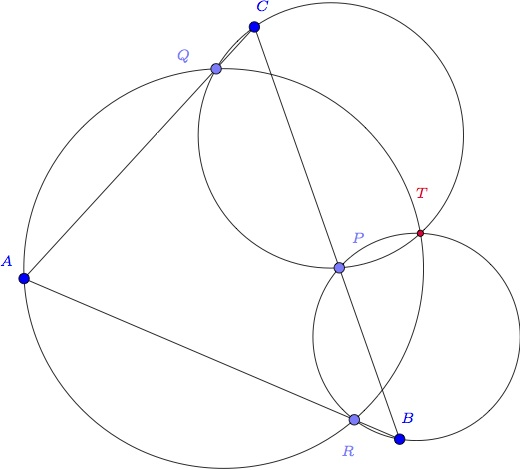
\includegraphics{../images/5Wyx-2}
\end{center}

(Les angles $\widehat{BRT}$ et $\widehat{BPT}$ sont supplémentaires dans la première figure, et égaux dans la seconde.)

Le second cas, celui où les deux premiers cercles sont tangents en $R$, se traite à l'aide du cas limite du théorème de l'angle au centre.
}
}
